%% custom vibs.tex
%% $Id: Genetischer Algorithmus.tex 28 2007-01-18 16:31:32Z bless $
%%

Da heutzutage beinahe jedes Ger{\"a}t ein Vibtarionsmotor verbaut hat, sei es das Handy, die Smartwatches oder Fitnessarmb{\"a}nder (uvm.), werde ich im folgenden auf einige aktuelle Technologien und deren Umsetzung der personalisierten Vibtationsmuster zu sprechen kommen. 

%% ==============================
\subsection{Taptic Engine}
%% ==============================
\label{ch:Grundlagen:sec:RelatedWork:subsec:TapticEngine}

Die Taptic Engine ist ein von der Firma Apple selbst entwickeltes Vibrationsmotor, dass heutzutage in nahezu allen Apple Produkten verbaut ist. Das erste Ger{\"a}t ,was die Taptic Engine bekommen hat, war die Apple Watch. Der Name \textbf{Taptic} bildet sich aus dem W{\"o}rtern "`Taktil"' und "`Haptisch"'. 
Trotz der neu Erfindung einer mechanischen R{\"u}ckmeldung, bietet Apple keine Personalisierung, wie lange eine R{\"u}ckmeldung f{\"u}r die Apple Watch erfolgen soll. Die Einstellungsm{\"o}glichkeiten an der Apple Watch ist lediglich die St{\"a}rke der Vibration. Diese ist in 3 St{\"a}rkestufen unterteilt. Meiner Ansicht nach kann man daher nicht wirklich von einer personalisierten Vibration sprechen. 

\begin{figure}[htbp] 
	\centering
	\begin{minipage}[t]{0.4\textwidth}
		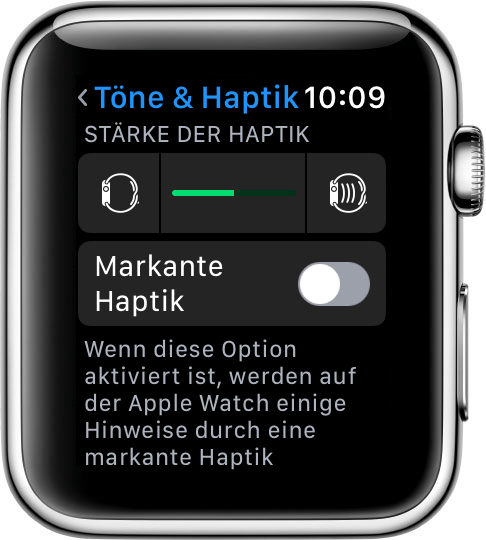
\includegraphics[width=\textwidth]{pics/applewatch.png}
	\end{minipage}
	\begin{minipage}[t]{0.4\textwidth}
		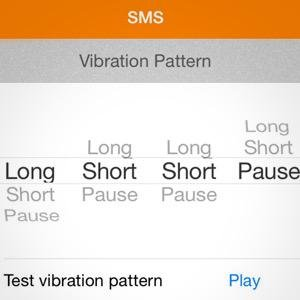
\includegraphics[width=\textwidth]{pics/martian.jpg}
	\end{minipage}
	\caption{Einstellungsmöglichkeit auf der Apple Watch (links) und in der Martian App (rechts)}
	\label{fig:Bild10}
\end{figure}

%\begin{figure}
%	\centering
%    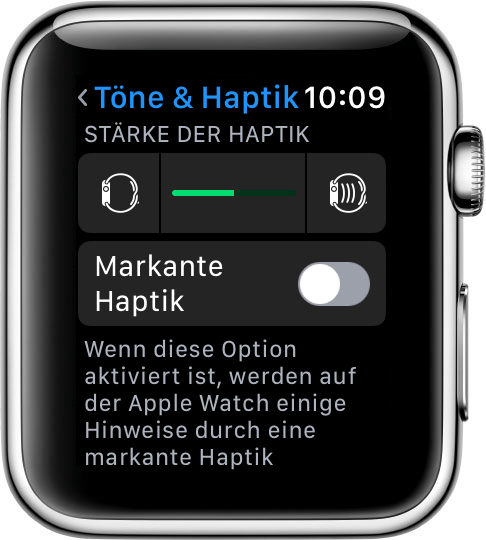
\includegraphics[width=\textwidth]{pics/applewatch.png}
%    \caption{Settings on the apple watch}
%    \label{fig:applewatch}
%\end{figure}
 
%% ==============================
\subsection{iPhone}
%% ==============================
\label{ch:Grundlagen:sec:RelatedWork:subsec:PersonalisierteVibration}

\begin{figure}
	\centering
    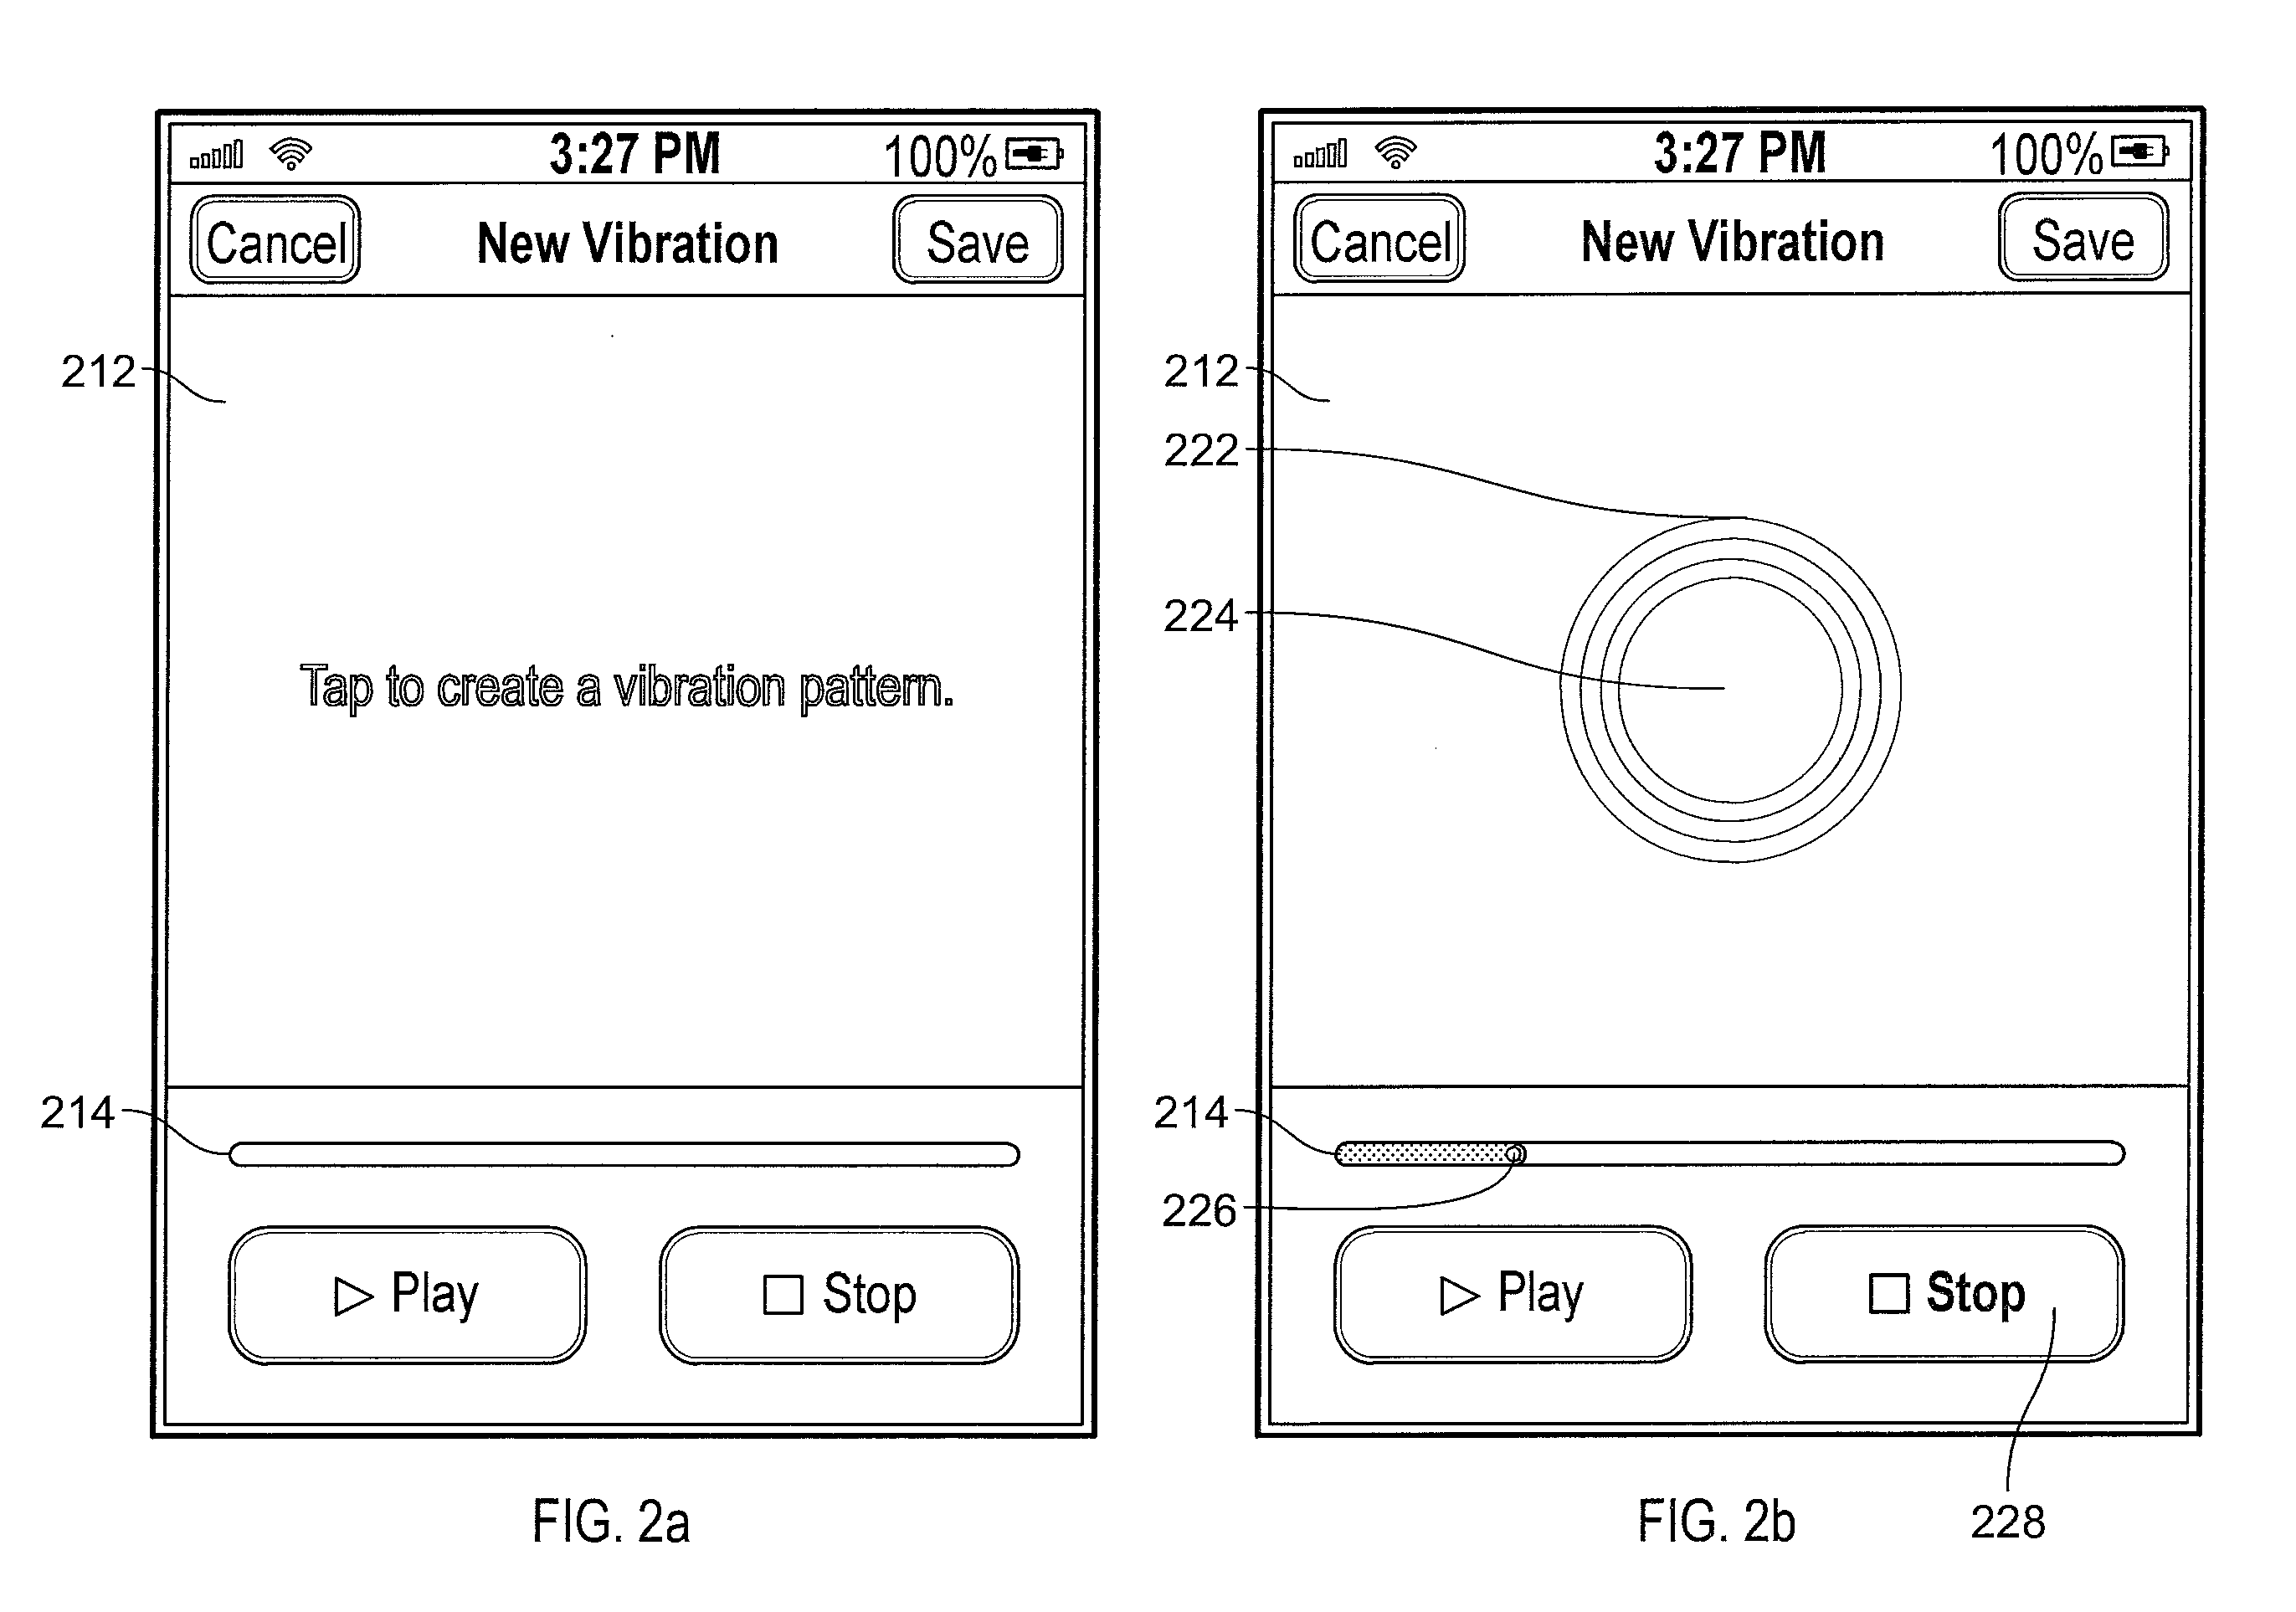
\includegraphics[width=\textwidth]{pics/iphone.png}
    \caption{Erstellung eigener Vibrationsmuster auf dem iPhone}
    \label{fig:iphone}
\end{figure}

Der Hersteller Apple hat auch bei dem iPhone eine M{\"o}glichkeit geboten, eigene Vibrationsmuster zu erstellen, jedoch mit Einschr{\"a}nkungen.
Wenn man in die jeweilige Einstellung der iPhones gelangt, erscheint das folgende Bild \autoref{fig:iphone}. 
Beim dr{\"u}cken auf das Display wird an der Stelle eine Vibration erzeugt. 
Man hat 10 Sekunden um ein eigenes Muster zu erzeugen, indem man wiederholt auf den Bildschirm dr{\"u}ckt. 
An der Stelle, an der man den Bildschirm ber{\"u}hrt hat, erscheint visuell um der Position ein Kreis. 
Die erzeugten Vibrationen werden in einer Leiste visuell angezeigt. 
Man kann sich beliebig viele Vibrationsmuster speichern, die bis zu 10 Sekunden lang sind. \cite{fleizach2016custom}

Die Einschr{\"a}nkung die man hier erwähnen muss ist, dass man die Vibrationsmuster nur f{\"u}r Systeminterne Funktionen benutzen kann. 
Dies bedeutet, dass man die Funktionen f{\"u}r Klingelt{\"o}ne, Nachrichtent{\"o}ne, Erinnerungshinweise, Kalenderhinweise (o.{\"a}.) hinzuf{\"u}gen kann. 
F{\"u}r eine andere Anwendung, die nicht im Betriebsystem integriert sind, ist das nicht m{\"o}glich. 
Somit k{\"o}nnen Benachrichtigungen von anderen Entwicklern keine eigene Vibrationsmuster erhalten. 
Trägt man das iPhone in der Hosentasche und es wird eine Benachrichtigunge einer Application empfangen, die nicht im System integriert ist, kann man anhand der Vibrationen des iPhones nicht unterscheiden welche Application dies gewesen ist.
%Daraus folgt, wenn das iPhone in der Hosentasche ist und ich eine Benachrichtigung von einer Application erhalte, die nicht im System integriert gewesen ist, kann man anhand der Vibrationen des iPhones nicht unterscheiden welche Application dies gewesen ist.
% kann man bei Benachrichtigungen von anderen Entwicklern nicht anhand der Vibrationen des iPhones  unterscheiden.

%% ==============================
\subsection{Martian Smartwatch}
%% ==============================
\label{ch:Grundlagen:sec:RelatedWork:subsec:PersonalisierteSmartwatch}

%\begin{figure}
%	\centering
%    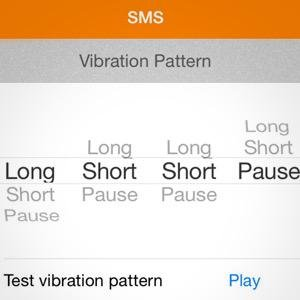
\includegraphics[width=\textwidth]{pics/martian.jpg}
%    \caption{possible settings on the martian watch}
%    \label{fig:martian}
%\end{figure}

Das Ger{\"a}t, dass es nach meiner Recherche am besten gel{\"o}st hat, ist eine Smartwatch von einem kleinen StartUp namens Martian. 
Das Startup hat eine Uhr hergestellt, mit der man mittels einer App auf dem Smartphone die Vibrationsmuster selbst anpassen kann. 
Die App unterst{\"u}tzt eine gro{\ss}e Anzahl an Applications, von anderen Herstellern, die Benachrichtigungen senden. 
Ein Vibrationsmuster f{\"u}r die Uhr kann man aus mit zu 4 Signalen auf der Uhr darstellen. 
Die Signale sind als Lang, Kurz und Pause festgelegt. 
Somit kann man mittels der Vibration der Uhr herausfinden, welche App gerade eine Benachrichtigung auf mein Handy gesendet hat. 
Die L{\"a}nge und St{\"a}rke eines Signals ist vom Hersteller festgelegt und kann nicht geändert werden.

%% ==============================
\subsection{Andere Hersteller}
%% ==============================
\label{ch:Grundlagen:sec:RelatedWork:subsec:PersonalisierteSmartwatch}
Bei sehr vielen Herstellern ist es aktuell noch gar nicht m{\"o}glich eigene Vibrationsmuster zu erstellen. 
Bei Android Ger{\"a}ten ist es aktuell so, dass man aus einer Menge von wenigen vordefinierten Vibrationsmustern sich nur einen ausw{\"a}hlen kann. 
Einige Entwickler haben dieses Problem erkannt und eigene Applikationen entwickelt die im Store ver{\"o}ffentlicht sind.





